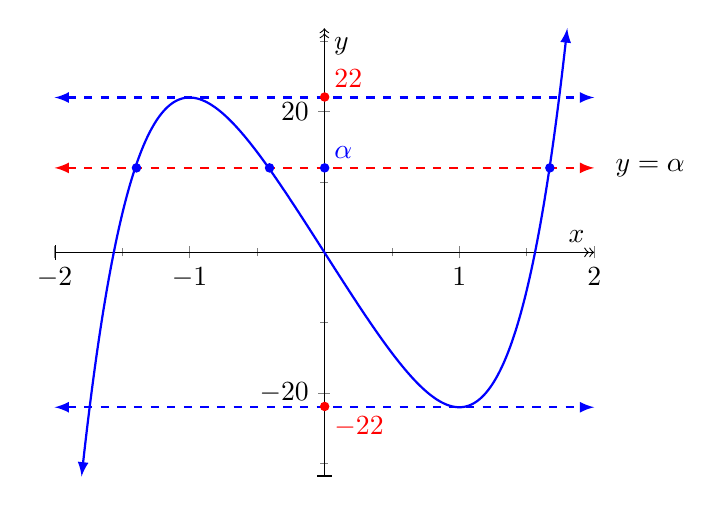
\begin{tikzpicture}
%\draw [very thin, style=gray!50, step=1] (-3,-2) grid (7,7);
\begin{scope}
\begin{axis}[ minor tick num=1, axis x line=middle, axis y line=middle, every inner x axis line/.append style= {|->>}, every inner y axis line/.append style= {|->>}, xlabel=$x$,ylabel=$y$ ]
\addplot[domain=-1.8:1.8,blue,thick,samples=500,latex-latex]{3*x^5+5*x^3-30*x};
\addplot[domain=-2:2,blue, thick,dashed,latex-latex]{22};
\addplot[domain=-2:2,blue, thick,dashed,latex-latex]{-22};
\addplot[domain=-2:2,red, thick,dashed,latex-latex]{12};
\end{axis}
 %\filldraw[red] (0,0) circle (1pt) node[below] {$O$};
 \filldraw [red] (3.43,4.82) circle (1.5pt) node[above right] {$22$};
\filldraw[red]  (3.43,0.89) circle (1.5pt) node[below right] {$-22$};
\filldraw[blue]  (3.43,3.92) circle (1.5pt) node[above right] {$\alpha$};
\filldraw (7,3.92) node[right] {$y=\alpha$};
\filldraw[blue]  (2.73,3.92) circle (1.5pt) node[above right] {};
\filldraw[blue]  (6.29,3.92) circle (1.5pt) node[above right] {};
\filldraw[blue]  (1.04,3.92) circle (1.5pt) node[above right] {};
\end{scope}
 
\end{tikzpicture}